It is assumed here that the formation of the 30S and 50S complexes are described and modeled somewhere else as well as for the metabolites.

\textcolor[rgb]{1.00,0.00,0.00}{Something equivalent to non coding DNA? Non coding codon???} \\
\textcolor[rgb]{1.00,0.00,0.00}{Put RBS (Ribosome Binding Site) somewhere in the mRNA properties.} \\
\textcolor[rgb]{1.00,0.00,0.00}{Mettre des propriétés sur la protéine qui devrait sortir du ribosome pour éventuellement prendre en compte des évènements sur la future protéine pendant la traduction (genre N-myristoylation, N-acyliation, euh non, ca c'est de la post traduction. Y a-t-il des trucs qui se passent sur la future proteine pendant la traduction?)} \\
\textcolor[rgb]{1.00,0.00,0.00}{Ecrire un truc à part pour la formation du ribosome = rRNA + protéines. En février 2009, la revue Nature a publié un article rédigé par des biophysiciens de l'Université de Montréal : ils y expliquent les mécanismes de formation de cette molécule qui peut contenir jusqu'à 300 000 atomes. Ces explications permettraient de mieux comprendre les mécanismes de création des êtres vivants.} \\
\textcolor[rgb]{1.00,0.00,0.00}{Mettre une propriété pour une mauvaise traduction: mauvais AA pendant la traduction.} \\

\bigskip

\textcolor[rgb]{1.00,0.00,0.00}{\Huge Regulation?}


\subsubsection{tRNA charging or loading}
\paragraph{Biological process} A tRNA has an anticodon which corresponds to a specific amino acid. There are 64 possibilities for a codon for twenty or so amino acids. Let's number the possibilities with $i$. Each one of these possibilities leads to a type of tRNA, $tRNA^i$. The mechanism of charging the tRNA is performed by an enzyme, an aminoacyl tRNA synthetase (aaRS), which is also specific to an anticodon sequence. The mechanism is described below:
$$
  \left\{
    \begin{array}{l}
      \reactionRev{aaRS^i + ATP}{aaRS^i_t}{}{} \\
      \reactionIrr{aaRS^i_t + AA^i}{aaRS^i_{cm}+PP_i+\ce{H+}}{}{} \\
      \reactionIrr{aaRS^i_{cm} + tRNA^i}{aaRS^i + tRNA^i_c + AMP}{}{} \\
    \end{array}
  \right.
$$
with the pyrophosphate anion $PP_i=\ce{P2O7^4-}$. Pyrophosphate anion is unstable in aqueous solution and hydrolyzes into inorganic phosphate $P_i=\ce{HPO4^2-}$. In short:
\begin{mdframed}[style=MyFrame]
$$
  \left\{
    \begin{array}{l}
    \reactionIrr{AA^i+ATP+tRNA^i}{tRNA^i_c+AMP+PP_i+\ce{H+}}{aaRS^i}{} \\
    \reactionIrr{PP_i + \ce{H2O}}{2P_i}{}{} \\
  \end{array}
  \right. .
$$
\end{mdframed}
Finally, note that during the elongation, a \ce{H2O} is consumed. If we pair both process, it is possible to write
\begin{mdframed}[style=MyFrame]
$$
  \reactionIrr{AA^i+ATP+tRNA^i}{tRNA^i_c+AMP+2P_i+\ce{H+}}{aaRS^i}{} \\
$$
\end{mdframed}
\textcolor[rgb]{1.00,0.00,0.00}{On en fait quoi du $P_i$?}
\textcolor[rgb]{1.00,0.00,0.00}{On en fait quoi du AMP? Mettre un cycle énergétique quelque part.}


\paragraph{Biological error} The authors are not aware of any biological error that can happen during tRNA loading.



\subsubsection{Initiation}
\paragraph{Biological process} The purpose of the initiation is to locate precisely the initiation $fMet$ amino acid at the Ribosome Binding Site where is located the start codon of the mRNA. The initiation is a complex mechanism that starts from the association of the initiation factors to the $30S$ complex and ends with the formation of the $70S$ complex via the binding of the $50S$ complex to the mRNA. The active steps are illustrated in Figure \ref{fig:initTranslate}.
\begin{figure}[hbtp]
  \centering
  % Requires \usepackage{graphicx}
  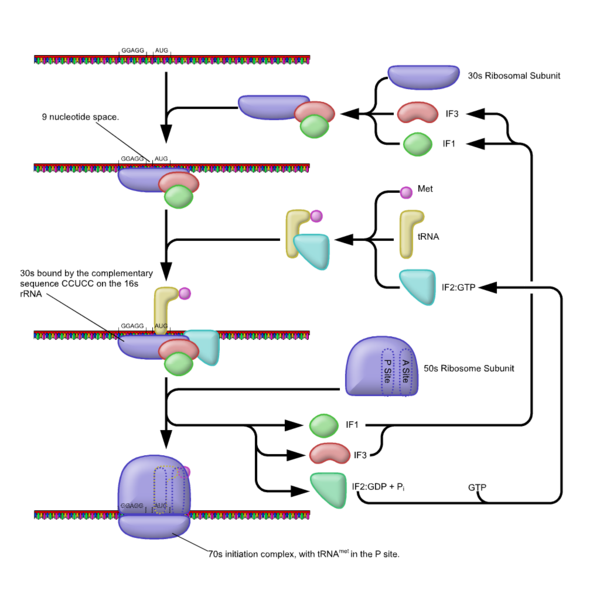
\includegraphics[width=15cm]{figure/prokaryoticTranslationInitiationFromWikibooks.png}\\
  \caption{Initiation of translation @Wikipedia}\label{fig:initTranslate}
\end{figure}
The steps are detailed hereafter:
%\begin{enumerate}
%  \item binding of the metabolites of $IF_3$, then $IF_1$ and finally a form $IF_2$ to the $30S$ complex, referred to as $30S_{312}$. The different forms of $IF_2$ are:
%  \begin{enumerate}
%    \item $IF_2$: the initiation factor without cofactor. The corresponding complex is referred to as $30S_{312}$ (it can be assumed that this does never happen),
%    \item $IF_{2a}$: the active form coming from the reaction $\reactionRev{IF_2+GTP}{IF_{2a}}{}{}$. The corresponding complex is referred to as $30S_{312a}$,
%    \item $IF_{2d}$: an inactive form coming from the reaction $\reactionRev{IF_2+GDP}{IF_{2d}}{}{}$. The corresponding complex is referred to as $30S_{312d}$,
%    \item $IF_{2p}$: an inactive form coming from the reaction $\reactionRev{IF_2+ppGpp}{IF_{2p}}{}{}$. The corresponding complex is referred to as $30S_{312p}$;
%  \end{enumerate}
%  \item the $30S$ complex then binds to the mRNA following
%  $$
%    \left\{
%      \begin{array}{l}
%%        \reactionRev{30S_{312}+mRNA}{m30S_{312}}{}{} \\
%        \reactionRev{30S_{312a}+mRNA}{m30S_{312a}}{}{} \\
%        \reactionRev{30S_{312d}+mRNA}{m30S_{312d}}{}{} \\
%        \reactionRev{30S_{312p}+mRNA}{m30S_{312p}}{}{} \\
%      \end{array}
%    \right.
%  $$
%  \item the $m30S_{312a}$ complex has a high affinity with charged tRNA with $fMET$ (denoted by $tRNA_{fMET}$) \textcolor[rgb]{1.00,0.00,0.00}{How does the charging of tRNA works?}. It is assumed that $m30S_{312p}$ does not allow this binding:
%      $$
%      \left\{
%        \begin{array}{l}
%          \reactionIrr{m30S_{312a}+tRNA_{fMET}}{mt30S_{312afMET}}{}{} \\
%          \reactionRev{m30S_{312d}+tRNA_{fMET}}{mt30S_{312dfMET}}{}{} \\
%        \end{array}
%      \right. ;
%      $$
%  \item $IF_3$ is then released:
%        $$
%      \left\{
%        \begin{array}{l}
%          \reactionRev{mt30S_{312afMET}}{mt30S_{12afMET}+IF_3}{}{} \\
%          \reactionRev{mt30S_{312dfMET}}{mt30S_{12dfMET}+IF_3}{}{} \\
%        \end{array}
%      \right. ;
%      $$
%  \item the $50S$ complex binds to form the $70S$ complex and $IF_1$ and $IF_2$ are released. Only an active form allows this binding:
%  $$
%    \reactionIrr{mt30S_{12afMET}+50S}{70S+IF_1+IF_{2d}}{}{}.
%  $$
%\end{enumerate}
%\noindent Note that the $tRNA_{fMET}$ is already at P-site so that the complex is ready for elongation.
\begin{enumerate}
  \item in parallel, the $30S$ complex binds to the $mRNA$ when the $IF_3$ and $IF_1$ have already binded to it whereas $IF_2$ binds with a co-factor and to a $tRNA^{fMet}$ (an $fMet$ charged tRNA):
    \begin{itemize}
    \item the $30S$ complex binds to the $mRNA$:
      \begin{enumerate}
      \item the binding of the initiation factors $IF_3$ and $IF_1$ to a $30S$ complex:
        $$
        \left\{
          \begin{array}{l}
          \reactionRev{30S+IF_3}{30S_3}{}{} \\
          \reactionRev{30S_3+IF_1}{30S_{31}}{}{} \\
          \end{array}
        \right.                                                                                                                                                 ,
        $$
      \item the binding of formed complex to the $mRNA$:
        $$
        \reactionRev{30S_{31}+mRNA}{m30S_{31}}{}{}{}
        $$
      \end{enumerate}
    \item the binding of the initiation factor $IF_2$ with a cofactor and to a $tRNA^{fMet}$: \textcolor[rgb]{1.00,0.00,0.00}{comment se forme le $tRNA^{fMet}$? Codon spécifique ou un truc différent? IF2 peut-il se binder a autre chose qu'un tRNAfMet ?}
      \begin{itemize}
      \item $IF_2$: the initiation factor without cofactor. It is assumed that $IF_2$ does not bind with a $tRNA^{fMet}$,
%        $$
%        \reactionRev{tRNA^{fMet}+IF_{2}}{tRNA_{2}^{fMet}}{}{} \\
%        $$
      \item $IF_{2a}$: the active form coming from the $GTP$ cofactor
        $$
        \left\{
          \begin{array}{l}
          \reactionRev{IF_2+GTP}{IF_{2a}}{}{} \\
          \reactionRev{tRNA^{fMet}+IF_{2a}}{tRNA_{2a}^{fMet}}{}{} \\
          \end{array}
        \right. ,
        $$
      \item $IF_{2d}$: an inactive form coming from the $GDP$ cofactor
        $$
        \left\{
          \begin{array}{l}
          \reactionRev{IF_2+GDP}{IF_{2d}}{}{} \\
          \reactionRev{tRNA^{fMet}+IF_{2d}}{tRNA_{2d}^{fMet}}{}{} \\
          \end{array}
        \right. ,
        $$
      \item $IF_{2p}$: an inactive form coming from the $ppGpp$ cofactor
        $$
        \left\{
          \begin{array}{l}
          \reactionRev{IF_2+ppGpp}{IF_{2p}}{}{} \\
          \reactionRev{tRNA^{fMet}+IF_{2p}}{tRNA_{2p}^{fMet}}{}{} \\
          \end{array}
        \right. ;
        $$
      \end{itemize}
    \end{itemize}
  \item the $m30S_{31}$ complex has a high affinity with charged tRNA with $fMet$ (denoted by $tRNA^{fMet}$). It is assumed that $tRNA_{2p}^{fMet}$ does not binds:
    $$
    \left\{
      \begin{array}{l}
      \reactionIrr{m30S_{31}+tRNA_{2a}^{fMet}}{mt30S_{312a}^{fMet}}{}{} \\
      \reactionRev{m30S_{31}+tRNA_{2d}^{fMet}}{mt30S_{312d}^{fMet}}{}{} \\
      \end{array}
    \right. ;
    $$
  \item $IF_3$ is then released:
    $$
    \reactionIrr{mt30S_{312a}^{fMet}}{mt30S_{12a}^{fMet}+IF_3}{}{} ;
    $$
%    $$
%    \left\{
%      \begin{array}{l}
%      \reactionIrr{mt30S_{312a}^{fMet}}{mt30S_{12a}^{fMet}+IF_3}{}{} \\
%      \reactionRev{mt30S_{312d}^{fMet}}{mt30S_{12d}^{fMet}+IF_3}{}{} \\
%      \end{array}
%    \right. ;
%    $$
  \item the $50S$ complex binds to form the $70S$ complex and $IF_1$ and $IF_2$ are released. Only an active form allows this binding:
    $$
    \reactionIrr{mt30S_{12a}^{fMet}+50S}{70S+IF_1+IF_{2d}+P_i+\ce{H2O}}{}{}.
    $$
\end{enumerate}
\noindent Note that the $tRNA^{fMet}$ is already at P-site of the $70S$ complex so that it is ready for elongation.

\medskip

In summary, we have the possible overall reactions:
\begin{mdframed}[style=MyFrame]
$$
  \left\{
    \begin{array}{l}
      \reactionRev{30S+IF_3+IF_1+mRNA}{m30S_{31}}{}{} \\
      \reactionRev{IF_2+GTP}{IF_{2a}}{}{} \\
      \reactionRev{IF_2+GDP}{IF_{2d}}{}{} \\
      \reactionRev{IF_2+ppGpp}{IF_{2p}}{}{} \\
      \reactionRev{IF_{2p}+tRNA^{fMet}}{tRNA_{2p}^{fMet}}{}{}{} \\
      \reactionRev{m30S_{31}+IF_{2d}+tRNA^{fMet}}{mt30S_{312d}^{fMet}}{}{}{} \\
      \reactionIrr{m30S_{31}+IF_{2a}+tRNA^{fMet}}{70S+IF_1+IF_{2d}+IF_3+P_i+\ce{H2O}}{}{}{} \\
    \end{array}
  \right.
$$
\end{mdframed}
\textcolor[rgb]{1.00,0.00,0.00}{On en fait quoi du $P_i$? Oui parce que là, avec le tRNA, ça en fait 3 déjà.}


\paragraph{Biological error} The authors are not aware of any biological error that can happen during translation initiation.



\subsubsection{Elongation}
\paragraph{Biological process} Elongation is the process of creating the protein by putting amino acid one by one. Roughly, the elongation is illustrated in Figure \ref{fig:elongationTranslate}
\begin{figure}[hbtp]
  \centering
  % Requires \usepackage{graphicx}
  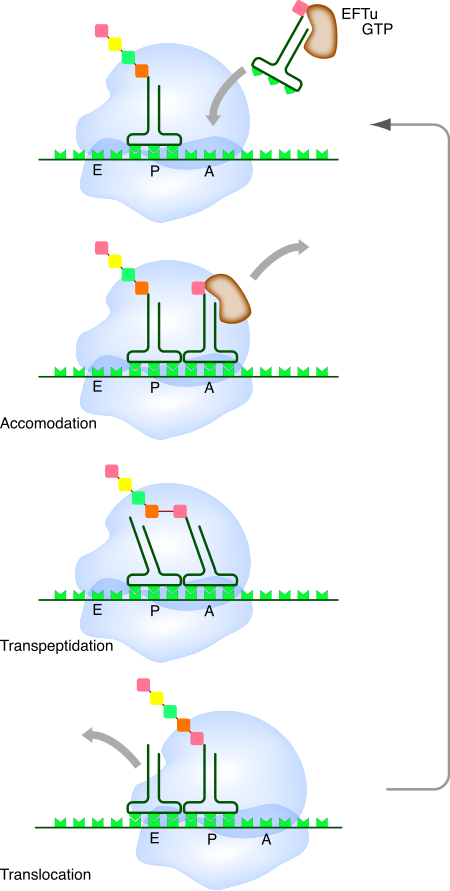
\includegraphics[width=9cm]{figure/proteinTranslationFromWikipediaModif.png}\\
  \caption{Elongation during translation @Wikipedia}\label{fig:elongationTranslate}
\end{figure}
and follows the steps:
\begin{enumerate}
  \item a charged tRNA binds to the A-site of the 70S complex;
  \item a peptide bond is formed between the new amino acid and the already here one at P-site;
  \item the ribosome translocate and the tRNA at E-site is released.
\end{enumerate}
The steps are explained hereafter, with the current (at A-site) codon being $i_0$:
\begin{enumerate}
  \item a tRNA (charged or uncharged) binds to the A-site of the 70S ribosomal complex. The affinity for cognate tRNA is higher the one for near-cognate tRNA. This tRNA is carried by the GTPase EF-Tu whose hydrolysis allows for the decoding between the mRNA codon and the tRNA anti-codon on the A-site. EF-Tu is released:
      \begin{enumerate}
        \item an EF-Tu with GTP ($EFTu_a$) binds to the tRNA (charged or uncharged)
          $$
            \left\{
            \begin{array}{l}
              \reactionRev{tRNA^i_c + EFTu_a}{EtRNA^i_{ca}}{}{} \\
              \reactionRev{tRNA^i + EFTu_a}{EtRNA^i_{a}}{}{} \\
            \end{array}
          \right.
          $$
        \item this tRNA then binds to the A-site of the 70S complex and EF-Tu is released (with GDP denoted $EFTu_d$)
          $$
            \left\{
            \begin{array}{l}
              \reactionRev{EtRNA^i_{a} + 70S}{Et70S^i_{a}}{}{} \\
              \reactionIrr{EtRNA^i_{ca} + 70S +\ce{H2O}}{t70S^i_{c} + EFTu_d + P_i}{}{} \\
            \end{array}
          \right.
          $$
          \textcolor[rgb]{1.00,0.00,0.00}{Proofreading (Olivier PhD)}
        \item as an aside, $EFTu_d$ is transformed back to $EFTu_a$ via a GTPase EF-Ts:
          $$
            \reactionIrr{EFTu_d + GTP}{EFTu_a + GDP}{EFTs}{}
          $$
      \end{enumerate}
  \item the peptide bond is formed via the elongation factor EF-P
    $$
      \left\{
        \begin{array}{l}
          \reactionRev{EFP + GTP}{EFP_a}{}{} \\
          \reactionIrr{t70S^i_{c} + EFP_a}{t70S^{+i} + EFP_d + \ce{H2O} + P_i}{}{} \\
        \end{array}
      \right.
    $$
    with $EFP_d$ being the GDP bounded form of $EFP$.
  \item translocation takes place via a elongation factor EF-G, a GTPase:
    $$
      \reactionIrr{t70S^{+i} + GTP+\ce{H2O}}{70S^{+} + tRNA^i + GDP + P_i}{EFG}{}.
    $$
%    EF-G is normally inhibited by fusidic acid, but resistance has emerged.
\end{enumerate}
\textcolor[rgb]{1.00,0.00,0.00}{From Olivier PhD, proofreading !}


\paragraph{Biological error} It s possible that the charged tRNA that comes to the A-site does not correspond to the anti-codon of the mRNA, that is $i\neq i_0$. It is possible that the protein produced is still correct due to the redundance of the amino acid coding. Otherwise it is assumed that the protein is non-functional.


\subsubsection{Termination}
\paragraph{Biological process} When the ribosome encounters a stop codon, it release the mRNA and the protein. In more details, when after the translocation step of elongation the ribosome encounters at its A-site a stop codon, a release factor (either $RF_1$ or $RF_2$ depending on the stop codon) binds. Note that tRNA are unable to recognize a stop codon. A final GTPase $RF_3$ hydrolysis allows the release of the protein. It can be summarized as follows:
$$
  \left\{
    \begin{array}{l}
      \reactionRev{RF_3 + GTP}{RF_{3a}}{}{} \\
      \reactionRev{70S + RF_1}{70S_1}{}{} \\
      \reactionRev{70S + RF_2}{70S_2}{}{} \\
      \reactionIrr{70S_1 + RF_{3a} + \ce{H2O}}{30S + 50S + protein + RF_1 + RF_{3d} + P_i}{}{} \\
      \reactionIrr{70S_2 + RF_{3a} + \ce{H2O}}{30S + 50S + protein + RF_2 + RF_{3d} + P_i}{}{} \\
    \end{array}
  \right.
$$
with $RF_{3d}$ being GDP bounded form of $RF_3$. The released protein can be 'correct' or not.

\textcolor[rgb]{1.00,0.00,0.00}{From Olivier PhD, last AA not in the protein.}


\paragraph{Biological error} The authors are not aware of any biological error that can happen during translation termination.

